\chapter{Using the debugger}
\thispagestyle{fancy}
\label{ch:debugging}

In the process of programming m-files, it is inevitable that errors, also known as bugs\index{bug}, will occur. \MATLAB{} provides some functionality to assist in \textit{debugging}\index{debugging} m-files. Two types of errors can occur in \MATLAB{} expressions: syntax errors\index{syntax error} and run-time errors\index{run-time error}. 

\section{Syntax errors}
Syntax errors (such as misspelled variable names, misspelled function names, missing quotes or parentheses, incorrect use of special characters, etc.) are found when \MATLAB{} is preparing to run the program. \MATLAB{} flags these errors immediately upon execution of the program and provides feedback about the type of error encountered and an estimate of the line number in the m-file where it occurs. Given this feedback and some experience, these errors are usually easy to spot.

\section{Run-time errors}
Run-time errors (programming errors such as zero divided by zero) are generally more difficult to find, because you can't tell just from looking at the code that it will generate an error. For example, your script may contain an addition {\tt A = B + C}, which you would not expect to contain an error. However, if the arrays {\tt B} and {\tt C} do not have the same size, \MATLAB{} will raise an error.

\section{Manual debugging}
In script m-files, you can monitor all calculation steps and variables by executing the command lines of the script m-file one by one in the command window. In this way, errors can usually be spotted quickly. In function m-files however, variables only exist as local variables living in their own part of the workspace away from the base workspace. This can make monitoring of the calculations and variables within functions very difficult.

There are several approaches to debugging function m-files. For simple problems, the easiest way to find bugs is to use a combination of the following:

\begin{enumerate}
\item {Remove semicolons within the function so that intermediate results are displayed in the command window;}
\item {Add statements that display variables of interest within the function;}
\item {Change the function m-file into a script m-file by placing a \% before the function definition statement at the beginning of the function m-file. When executing as a script file, the workspace is the \MATLAB{} workspace, and thus it can be interrogated after the error occurs. Declare input variables in the Command Window, otherwise they won't be present in the workspace;}
\item {Inserting a {\tt pause}\index{pause@\texttt{pause}} or {\tt keyboard}\index{keyboard@\texttt{keyboard}} command (e.g. in loops) enables you to view changes in your variables step by step (Refer to the documentation for the use of these functions).}
\end{enumerate}

\noindent When an m-file consists of multiple functions, or functions are called within functions, these methods are often not enough to efficiently debug your programs. For such problems, you must use the \MATLAB{} Debugger.


\section{Debugging in the Editor}
\begin{action}
Use the editor to open `000\_debugscript.m' and `000\_pfilt.m' (located in the folder `\textbackslash{}ch09\_debugging'). Click on \guitext{File} in the editor's menu and select \guitext{Save as\ldots}.
\end{action}


\begin{action}
Substitute your own last name for the zeros in the filenames.
\end{action} 

\begin{action}
Adapt the function call of {\tt 000\_pfilt} in {\tt 000\_debugscript} in accordance with the new name of the function m-file.
\end{action}


\noindent {\tt debugscript} is a simple program that uses the function {\tt pfilt} to filter a data set based on the deviation from the mean. However, the program is not functioning properly. Unfortunately, it is always very difficult to trace the bugs in someone else's program. You will need the \MATLAB{} debugger to help you.


\begin{action}	
Check for errors in the script {\tt debugscript} by running it from within the m-file editor.
\end{action}

\begin{action}
To be able to use the Debugger effectively, you need to arrange the GUI in such a way that you can see the editor window as well as the command window and the workspace. An easy way to do so is by clicking the \guitext{Dock Editor}-menu item under \guitext{Desktop} in the m-file editor's menu (see Figure \ref{fig:dock-editor}).
\end{action}


\begin{figure}[!htb]
  \centering
    \fbox{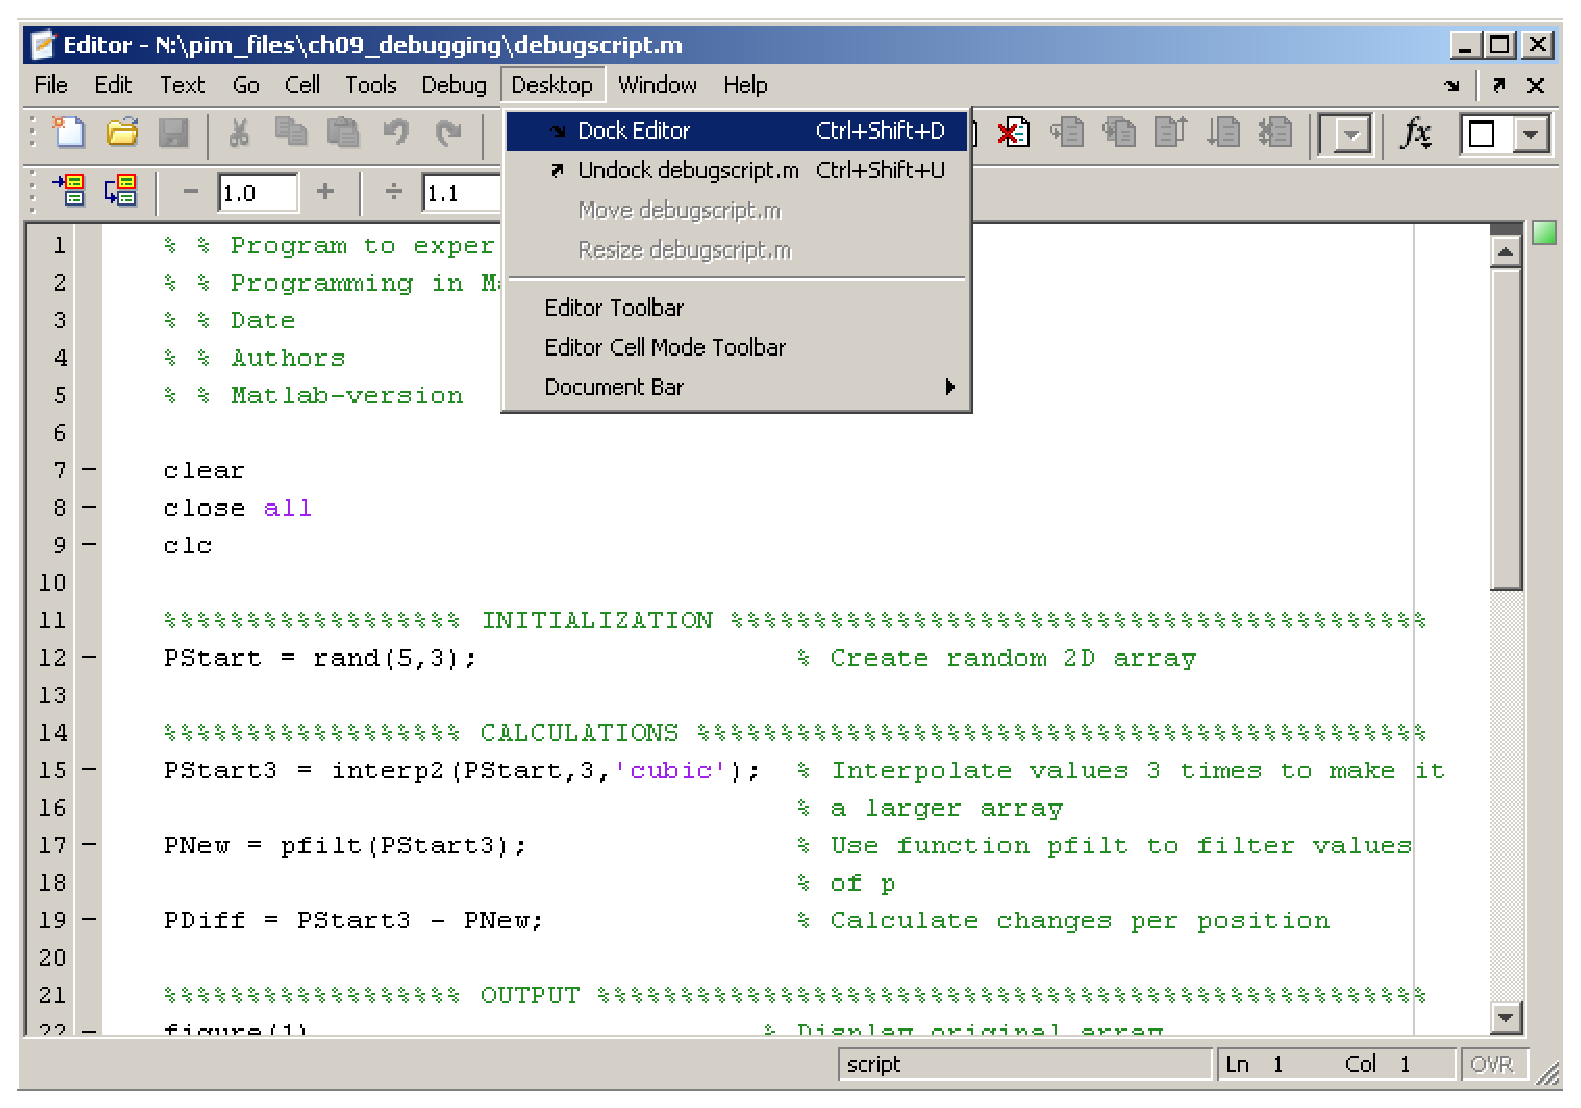
\includegraphics[width=1.0\textwidth]{./../eps/dock-editor.eps}}
  \caption{Docking the m-file editor.}\label{fig:dock-editor}
\end{figure}






\noindent Two errors occur somewhere in {\tt pfilt}. Because the variables in {\tt pfilt} live in the function workspace, monitoring of these variables is not straightforward. You can use the debug options in the Editor to trace and fix these errors. 

Note: to be able to use the debugging functionality, make sure that you have started the m-file editor from the command window using the {\tt edit} command. Also, if the editor window has been docked into the \MATLAB{} window, make sure that it is the active window by clicking anywhere in your m-file.

In order to use the debugger, you have to set breakpoints first. These breakpoints define where calculations will be (temporarily) stopped in the debug mode. You can set a breakpoint by clicking on one of the dash signs in the m-file editor's margin. Alternatively, you can move your cursor to a line and press the F12 button to set a breakpoint on that line. If you want, you can set multiple breakpoints. After a breakpoint has been set, a marker appears in the margin on that line (see Figure \ref{fig:set-breakpoint}). The color of this marker can be red or gray. If it is red, that means that the script in which your breakpoint has been set, was not changed since you saved it. If it is gray, that means that you have changed your m-file since the last time you saved it. 

\hintbox{Before running your file, you should always make sure that you saved it.}


\begin{figure}[!ht]
  \centering
    \fbox{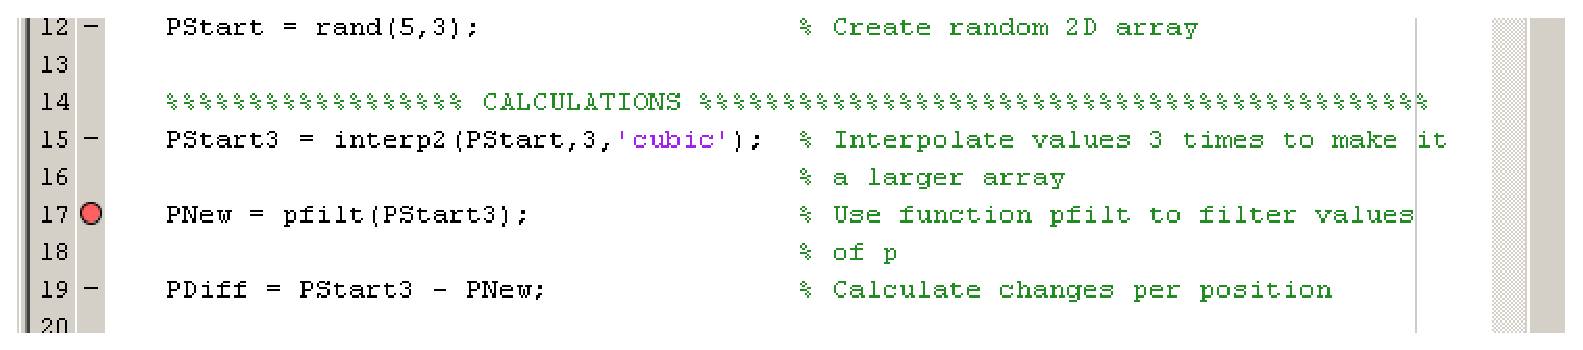
\includegraphics[width=1.0\textwidth]{./../eps/set-breakpoint.eps}}
  \caption{A breakpoint has been set.}\label{fig:set-breakpoint}
\end{figure}


\noindent By pressing F5 or clicking the \guitext{Run} button, the commands in the active m-file will be evaluated line by line until the end of your m-file is reached, or until the first breakpoint, whichever comes first. Breakpoints are usually set a few lines up from where you suspect an error. If you don't have any idea as to where an error occurs, you can set your breakpoint on the first line of the file. If you press F5 when any breakpoints exist in your m-file or in one of the functions it uses, \MATLAB{} will go to the debug mode. In the command window, the {\tt $>>$} is changed to {\tt K$>>$} to indicate the debug mode ({\tt K} for `keyboard'). If the commands in your m-file can be evaluated successfully up to the point where the breakpoint has been set, a green arrow appears on the breakpoint's line (see Figure \ref{fig:run-to-breakpoint}). After the breakpoint is reached, control is returned to the user and variables can be checked and commands entered at the prompt.

\begin{figure}[!ht]
  \centering
    \fbox{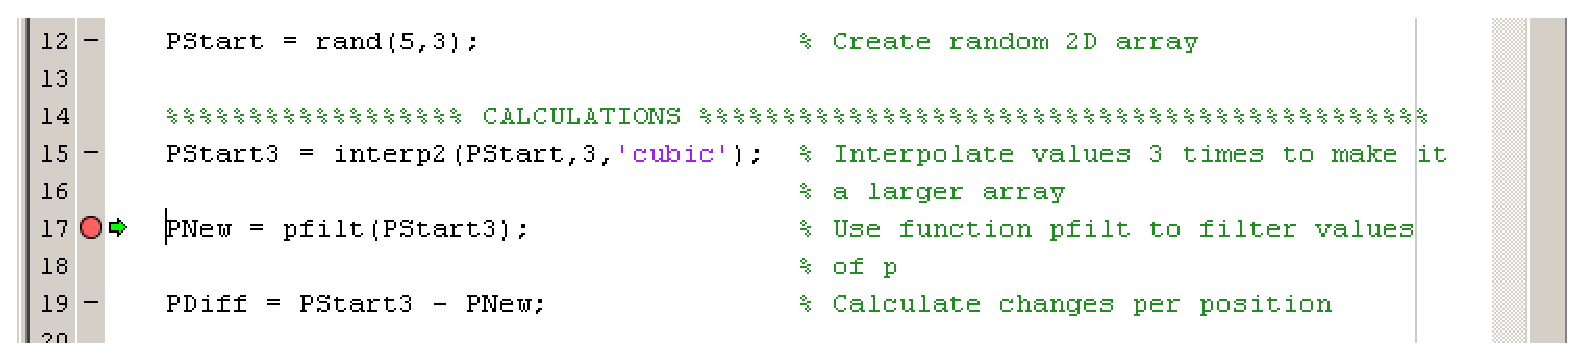
\includegraphics[width=1.0\textwidth]{./../eps/run-to-breakpoint.eps}}
  \caption{{\tt debugscript} has been evaluated successfully up to the breakpoint.}\label{fig:run-to-breakpoint}
\end{figure}

\vspace{1em}
\noindent Up to this point, debugging has been very similar to simply entering your commands one by one at the prompt. However, as soon as one of those commands happens to be a function (in which an error occurs), you will not be able to monitor the variables in the function's workspace by simply entering them at the prompt, since a function is somewhat like a black box: only the function's output arguments are returned to the base workspace. Because you cannot see the changes in the function's variables, finding the error in your function can become very difficult. The debugger, however, offers some useful tools to assess where the error is coming from.

If a breakpoint has been set and the commands can be evaluated successfully up to the breakpoint (in other words: if you have a green arrow), you can use \guitext{Step} from the \guitext{Debug} menu to go through your m-files line by line. Alternatively, you can press the F10 button. 

\begin{action}
Set a breakpoint at the very first command line (i.e. next to {\tt clear}) and run through your file line-by-line with the step function. Monitor how new variables are added to your workspace while you step through it.
\end{action}
\hintbox{You might have to right-click your workspace window and select \guitext{Refresh} to see the changes to your variables.}
\noindent If you try to step past the function call line at line 17, you will notice that \MATLAB{} returns an error. Apparently, the error is generated by some command used in the {\tt pfilt} function. Besides stepping through your m-file line-by-line by pressing F10, you can also step into functions with the input arguments that were calculated in the script.

\begin{action}
Set a breakpoint at the function call line of {\tt pfilt} and run your script m-file up to that point. List the variables that are present in your workspace.
\end{action}

\begin{action}
Now, select \guitext{Step in} from the \guitext{Debug} menu (or, equivalently, press F11) to step into the {\tt pfilt} function with the input argument(s) necessary for the successful execution of {\tt pfilt}.
\end{action}

\begin{action}
The green arrow should now be right next to the first command line in {\tt pfilt}. Compare your workspace with the list of variables you made a moment ago. Where did all the variables go? And where did {\tt In01} come from? What information does it contain?
\end{action}



\noindent The great advantage of using \guitext{Step in} is that the workspace will contain the locally declared variables, which enables the explicit, step-by-step monitoring of your variables, even within function m-files.

 
\hintbox{Pressing `F5' or clicking the \guitext{Run} button when the active m-file is a function, will return an error:\newline\newline
{\tt ??? Input argument \squote{In01} is undefined.\newline\newline}
This is because trying to run a function on its own will cause the function's input arguments (in this case {\tt In01}) to remain undefined.
}
\noindent If you step into a function, the green arrow in the parent m-file (in this case {\tt debugscript}) changes into a white arrow (see Figure \ref{fig:breakpoint-white-arrow}). This indicates that {\tt debugscript} is not the file that you are currently in. Therefore, any variables displayed in the workspace window do not belong to this (parent) m-file. 


\begin{figure}[!ht]
  \centering
    \fbox{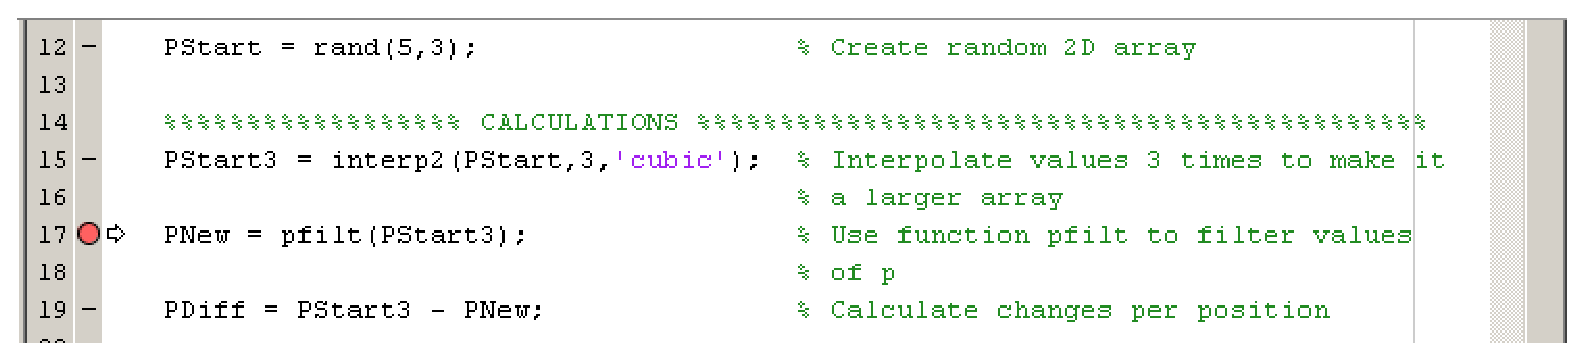
\includegraphics[width=1.0\textwidth]{./../eps/breakpoint-white-arrow.eps}}
  \caption{A white arrow in the parent m-file shows that it is not the active file.}\label{fig:breakpoint-white-arrow}
\end{figure}


\begin{action}
Use the \guitext{Step} function in {\tt pfilt} and check your workspace. Let the debugger execute command lines in {\tt pfilt} one at a time and continue to monitor the variables in your workspace. Monitoring of the variables in the workspace involves:
\begin{enumerate}
\item variable values;
\item variable names (pay attention to lowercase/uppercase)
\item variable dimensions (check the workspace column 'size') or type {\tt >> whos}
\item variable class (what is the data type of the variable under consideration?) For an overview of data classes, check Chapter \ref{ch:arrays}.
\end{enumerate}
\end{action}

\begin{action}
What problem arises when {\tt MinCrit} and {\tt MaxCrit} are calculated? What is the reason for this problem? Alter the command lines to solve this problem.
\end{action}

\noindent You have now corrected one of the errors in {\tt pfilt}. However, when running {\tt debugscript}, \MATLAB{} still returns an error message. Considering the output arguments of the function {\tt pfilt}, what command would you expect to be on the last line of this m-file?

\begin{action}
Correct the last error in {\tt pfilt}. Use the debug tools if necessary.
\end{action}


\noindent \guitext{Exit Debug Mode} from the \guitext{Debug}-menu will exit the debug session and invoke the normal mode indicated by the $>>$ sign. The debug mode can be exited at any time during debugging.

\hintbox{The \guitext{Stop if errors/warnings\ldots} in the \guitext{Debug} menu allows you to stop calculations right before an error or warning occurs. This functionality can be especially helpful when debugging loops.}


\noindent Before proceeding with the next chapter, make a review of the concepts covered in Chapters \ref{ch:math-functions}--\ref{ch:debugging}.


